\subsection{Methodology}
For latency benchmarking, we employed both \textit{iPerf3} and \textit{sockperf} \cite{sockperf}. 
Sockperf is a network benchmarking utility capable of measuring the latency of packets with a 
sub-nanosecond resolution. It introduces minimal overhead by leveraging the Time Stamp Counter (TSC) 
registers that count the number of CPU cycles for measuring latency \cite{sockperf}. 
Sockperf requires a client-server setup as well: the client sends mutliple packets to the server
, receives responses and records the \ac{RTT} for each packet. 
The tool provides different options to visualize the results with varying granularity. 
A CSV file is generated listing the send and response times for each individual packet,
along with a report of the average latency and key metrics such as the 90th and 99th percentile. \\
The objective of the latency experiment was to evaluate the effect of increasing aggregate throughput 
utilization of neighbors on the latency of the test node. The experiment is structured as 
follows.
\begin{figure}[H]
  \centering
  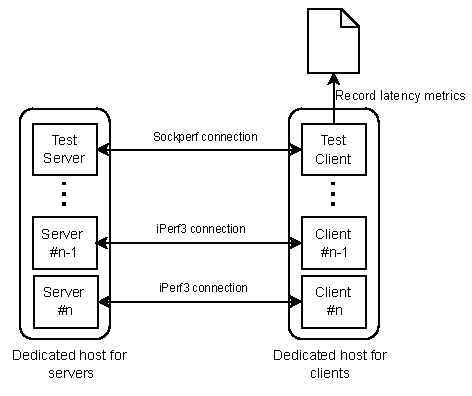
\includegraphics[width=11cm, height=8.5cm]{figures/latexp}
  \caption{Throughput contention experiment}
  \label{fig:latexp}
\end{figure}
\noindent
Similar to the throughput experiment, we deploy two dedicated hosts, 
one hosting all clients and one hosting all servers. Initially, only the client test node 
and its corresponding server are created. We measure the latency between them and record it as a baseline 
value. After that, we deploy all the remaining clients and incrementally increase their aggregate 
throughput usage in 1 Gbit/s steps (or smaller as we notice the presence of latency degrdation).
This is possible through an iPerf3 functionality that allows the specification of an exact throughput 
value for the client, allowing us to control the aggregated throughput of the neighbors.
After each step, i.e. increase, we measure the latency between the test client node and 
the test server using sockperf with the ping-pong option. The results are then recorded locally on the 
client side. 
Since all dedicated hosts, including the client test node and server, are located within 
the same \ac{AZ} (See Chapter \ref{chapter:infra}),
external latency variability is minimized, allowing for a better identification of latency 
degradation caused by increased throughput usage of the neighbors. \\ 